\documentclass[11pt, a4paper]{article}

\usepackage{graphicx}
\usepackage[a4paper,top=3cm,bottom=2cm,left=2cm,right=2cm,marginparwidth=1.75cm]{geometry}
\usepackage[english]{babel}
\usepackage[utf8x]{inputenc}
\usepackage{subfig}
\usepackage{amsmath}
\usepackage{amssymb}
\usepackage{array}

\graphicspath{ {./images} }
\newcommand*{\qed}{\hfill\ensuremath{\quad\square}}%
\newcommand*{\rad}{\ensuremath{\,\text{rad}}}
\newcommand*{\R}{\ensuremath{\mathbb{R}}}

\makeatletter
\renewcommand*\env@matrix[1][*\c@MaxMatrixCols c]{%
  \hskip -\arraycolsep
  \let\@ifnextchar\new@ifnextchar
  \array{#1}}
\makeatother

\newtheorem{theorem}{Theorem}

%------------------------------------------------
%Templates for images and figures
% \begin{figure}[h]
%   \centering
%   \subfloat[caption 1]{{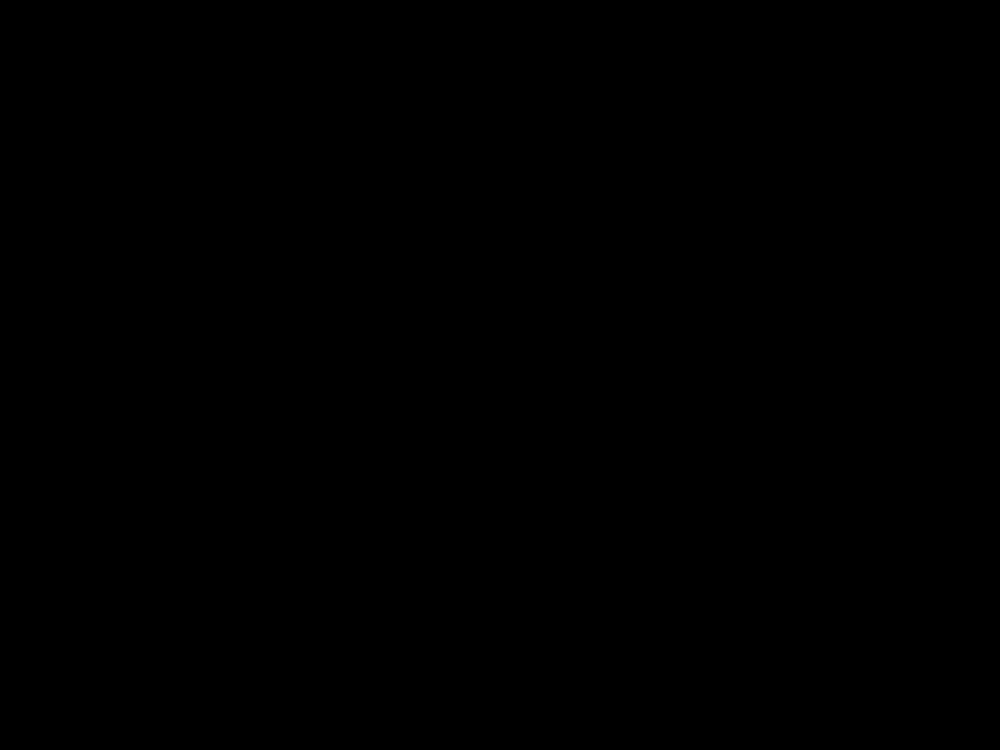
\includegraphics[width=30mm]{images/placeholder.png}}}%
%   \qquad
%   \subfloat[caption 2]{{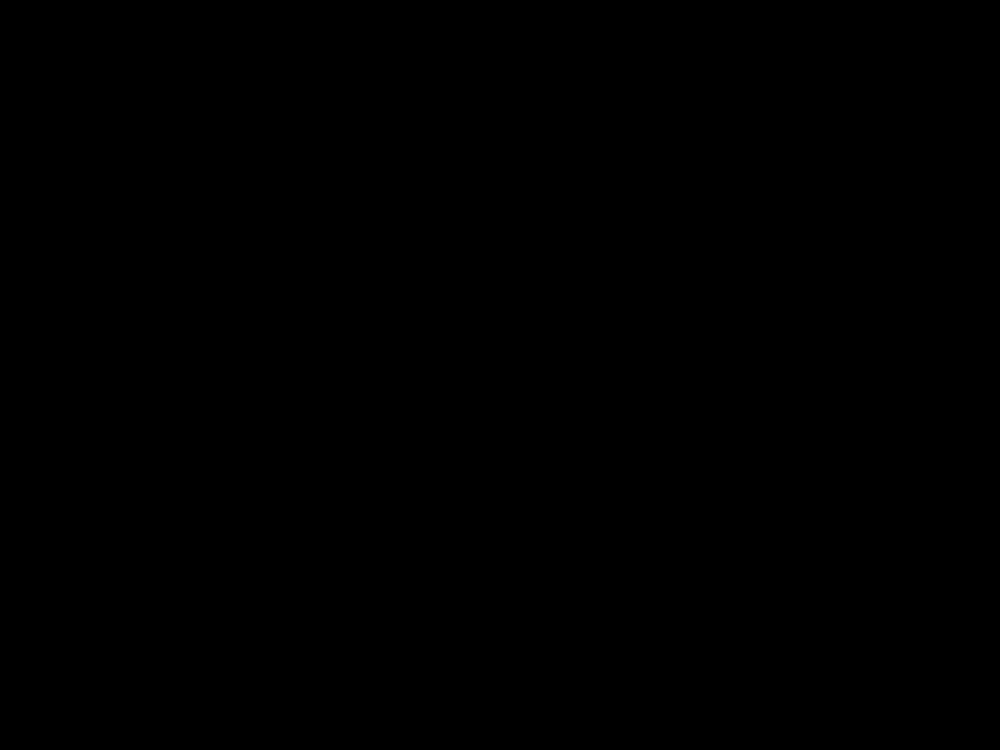
\includegraphics[width=30mm]{images/placeholder.png}}}%
%   \caption{Description}
% \end{figure}

% \begin{figure}[h]
%   \centerline{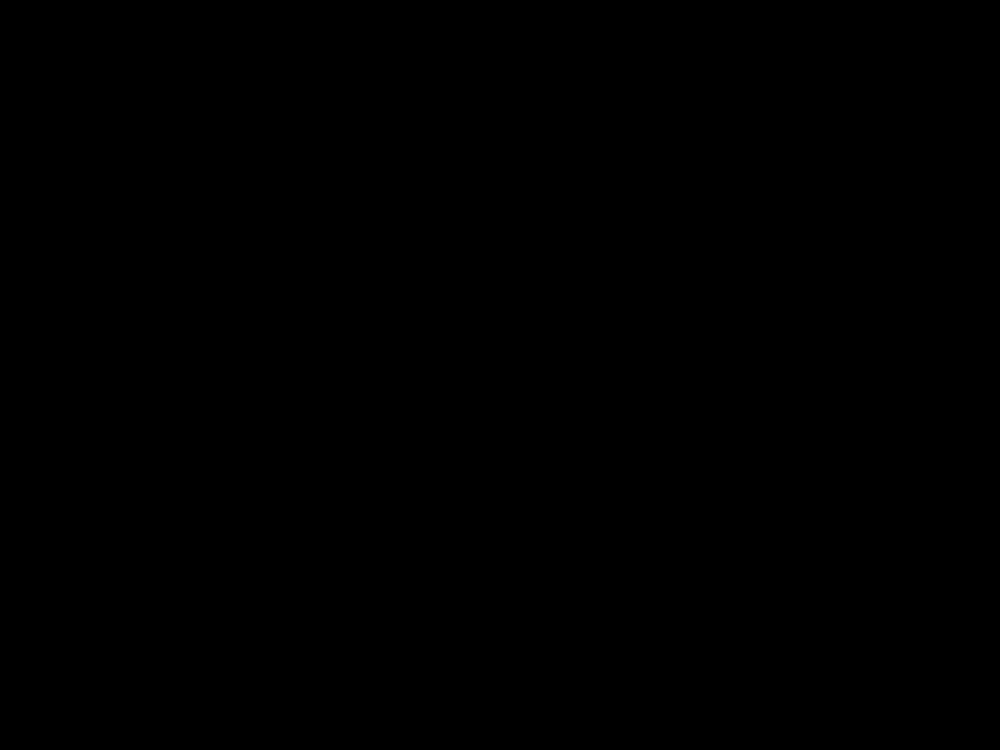
\includegraphics[width=50mm]{images/placeholder.png}}
%   \caption{Description}
% \end{figure}
%-----------------------------------------------

\begin{document}
\section{Thermofluids Lecture 1: Thermodynamic systems (20/04/2020)}


\subsection{Units used in the course}
Thermodynamics is the study of heat and energy transfer. There are a number of units which will commonly be found when studying thermodynamics. These are:
\begin{itemize}
  \item Energy: $J = Nm = Ws$
  \item Power: $W = J/s$
  \item Pressure: $Pa = N/m^2$
  \item Mass: $kg$
  \item Temperature: $K$ or $^\circ C$ (Kelvin is preferred)
\end{itemize}
Some other common important units are:
\begin{itemize}
  \item $1 Bar = 10^5 Pa = 100 kPa$
  \item $1 kWh = 3600 kJ$
  \item $1 kCal = 4.18 kJ$
\end{itemize}


\subsection{Definitions of terms used in the course}
\begin{itemize}
  \item \underline{System:}
\end{itemize}
A system is all the matter that is considered when analyzing a given problem. A system is defined by it's boundary. Systems can be either open or closed. Open or closed refers to whether mass can pass throught the boundary of a system. Thus for an open system matter can pass through the system boundary. For closed systems this is not the case.\\

\begin{table}[h!]
  \begin{center}
    \caption{The flows of work heat and mass for open and closed systems}
    \label{tab:table1}
    \begin{tabular}{l|c|c}
      \textbf{ } & \textbf{Closed} & \textbf{Open}\\
      \hline
      diabatic & 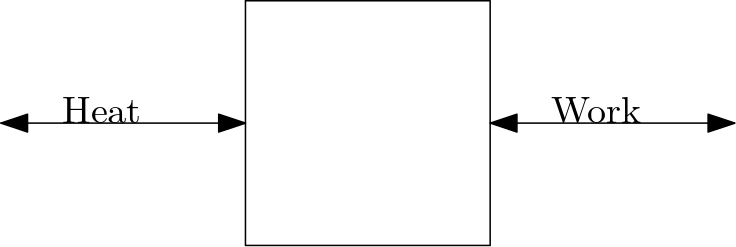
\includegraphics[ width=30mm]{images/Closed_diabatic.png}
               & 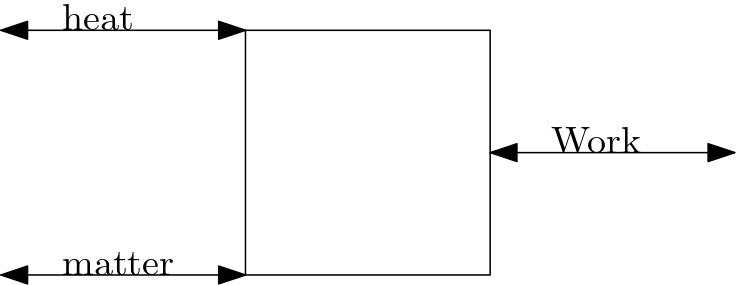
\includegraphics[ width=30mm]{images/Open_diabatic.png}\\
      
      adiabatic&\qquad \enspace 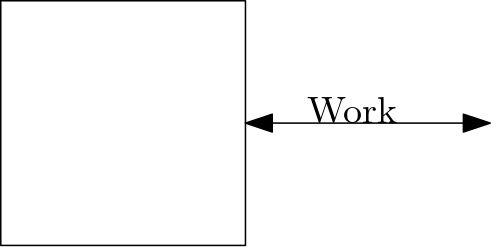
\includegraphics[ width=20mm]{images/Closed_adiabatic.png}
               &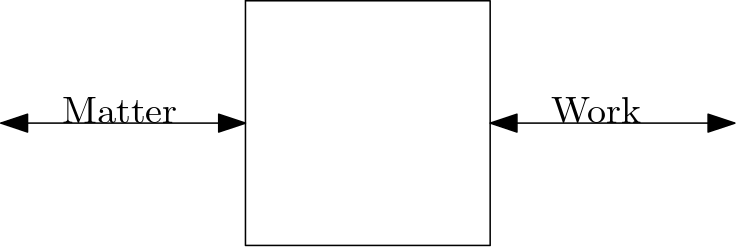
\includegraphics[ width=30mm]{images/Open_adiabatic.png}\\

      isolated &\includegraphics[ width=10mm]{images/isolated.png} & \\
    \end{tabular}
  \end{center}
\end{table}

\begin{itemize}
  \item \underline{continuum:}
\end{itemize}
In thermodynamics matter in considered to be a continuum. This means all matter is observed from a purely macroscopic scale. This means that the density at a single point can be defined as follows:
\begin{equation}
  \rho = \lim_{V \to V'}(\frac{m}{V})
\end{equation}
Where $V'$ is the smallest value for which the ratio $\frac{m}{V}$ excsits.\\

\begin{itemize}
  \item \underline{Thermodynamic equilibrium:}
\end{itemize}
An isolated system will eventually reach a time independent state. This final state is referred to as thermodynamic equilibrium. Classical thermodynamics only considers equilibrium states, and not how these states are reached. The analysis of how these states are reached is often part of statistical mechanics.\\

\begin{itemize}
  \item \underline{State variables or properties:}
\end{itemize}
The state of a system is defined by a small number of variables called the state variables. An example of this is the displacement and velocity of a system in dynamics. A property of a system is independent of the way a state is reached. The magnitude of a change in property only depends on the initial and final states of a system.\\

\begin{itemize}
  \item \underline{intensive, extensive and specific properties:}
\end{itemize}
\textbf{Intensive} properties do not change when the system is changed in size (e.g. Temperature and pressure). \textbf{Extensive} properties change proportional to the size of the system (e.g. mass, volume, energy). Extensive properties can be turned into intensive properties if described per unit of mass (or kmol). These are called \textbf{specific} properties. Examples of specific properties are specific volume and specific weight:
\begin{gather}
  v = \frac{V}{m},\; \bar{v}=vM\\
  \gamma_s = \rho g
\end{gather}
Where:
\begin{flalign*}
  &v, \bar{v} = \text{Specific volume } [m^3/kg], [m^3/kmol] &&\\
  &M = \text{Molar mass } [kg/kmol]\\
  &\gamma_s = \text{Specific weight} [N/m^3]\\
\end{flalign*}

\begin{itemize}
  \item \underline{Thermodynamic process:}
\end{itemize}
A process is defined as a change of state in a system. In classical thermodynamics we only consider the change from one equilibrium state to another equilibrium state. When the initial and final state in a system are identical the process is a cylce.

\begin{itemize}
  \item \underline{Quasi-static process:}
\end{itemize}
A process is considered to be quasi-static if it is reversible. These processes are generally very slow (less then the speed of sound).


\subsection{Pressure}
When talking about pressure in thermodynamics we usually refer to fluid or gas pressure. This can be thought of as the normal force exerted by a fluid per unit of area. Pressure measurements can either be absolute or relative to atmospheric pressure. Absolute pressure is measured relative to absolute vacuum (i.e. $p=0 Pa$). Gage pressure of measuring devices however is usually, for the sake of convenience measured relative to the atmospheric pressure. Thus in general:
\begin{equation}
  p_{abs} = p_{gage} + p_{atm}
\end{equation}
Fluid pressure variates with depth. Why this becomes apparent when considering a free body diagram of a body of fluid. When considering a point lower in the body the weight of the column of water above said point will have a much greater weight, thus increasing pressure. We can assume the density to be constant since liquids are generally incompressible. Because of this the following equation describes the pressure at any depth in a body of fluid:
\begin{equation}
  p_{gage} = \rho g \Delta z
\end{equation}
When considering very large depths the tremendous amount of pressure can sometimes make it so the approximation of $\rho$ being constant no longer holds. In this case we divide out $\Delta z$ and take the limit of $\Delta z \to 0$ which yields:
\begin{equation}
  \frac{dp}{dz} = -\rho g
\end{equation}
Which can be written in the form of an integral as:
\begin{equation}
  p = -\int_1^2 \rho g\,dz
\end{equation}


\subsection{Measurement of pressure}
Atmospheric pressure is usually measured with a barometer. It reads the pressure at any given place relative to the standard atmospheric pressure. The mathematics describing barometers is not that interesting and in general fairly trivial.\\
A different device for measuring pressure is a manometer. It uses a column of fluid, usually bent in a long U shape to compare the pressure at the 2 ends of the device. How much the fluid moves up allows us to compute the pressure of the gas going into the device relative to the atmospheric pressure. The figure below shows a basic manomete. The following equation describes the pressure of the gas:
\begin{equation}
  p_1 = p_2 = p_{atm} + \rho gh
\end{equation}

\begin{figure}[h]
  \centerline{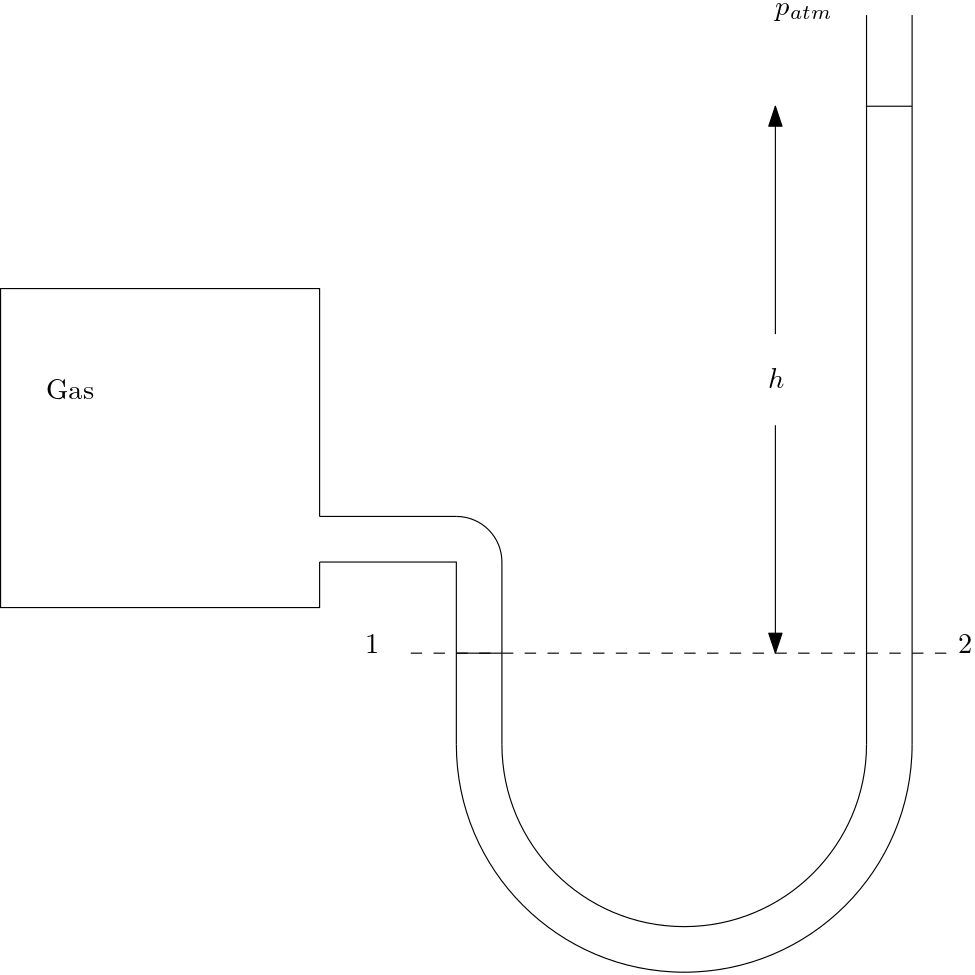
\includegraphics[width=50mm]{images/manometer.png}}
  \caption{A basic manometer design}
\end{figure}

\end{document}